%% Short IEEE conference paper: an accessible introduction to Observation Theory
%% through a single, clean case study -- ZooKeeper local-read staleness.
%% Reuses ot-replication-freshness.bib (same directory).
\documentclass[conference]{IEEEtran}
\usepackage[T1]{fontenc}
\usepackage[utf8]{inputenc}
\usepackage{amsmath,amssymb}
\usepackage{booktabs,array}
\usepackage{graphicx}
\newcolumntype{L}[1]{>{\raggedright\arraybackslash}p{#1}}
\newcolumntype{C}[1]{>{\centering\arraybackslash}p{#1}}
\usepackage{xcolor}
\usepackage[colorlinks=true,linkcolor=blue,citecolor=blue,urlcolor=blue]{hyperref}

\newcommand{\PC}{P_{\mathcal{C}}}
\newcommand{\tr}{\operatorname{tr}}
\newcommand{\fc}{\mathrm{FC}}

\begin{document}
\title{What \texttt{sync()} Certifies: A Consumer-Relative,\\ Witnessed Reading of ZooKeeper Staleness}

\author{\IEEEauthorblockN{Andrew H. Bond}
\IEEEauthorblockA{Department of Computer Engineering\\
San Jos\'e State University, San Jos\'e, CA, USA\\
andrew.bond@sjsu.edu}}
\maketitle

\begin{abstract}
A ZooKeeper client may read from any server, and a follower answers from its own
applied state---so a local read can be stale. ZooKeeper offers \texttt{sync()} to
force a read to reflect the latest committed state. We use this familiar
mechanism as a compact introduction to \emph{Observation Theory} (OT): the thesis
that reliability is a property of the relation between a system's error and
\emph{what a particular consumer reads}, and that any honest freshness claim needs
an independent \emph{witness}. In OT terms a local read is a \emph{certificate}
(this follower is fresh enough), the ZooKeeper transaction id (\texttt{zxid}) is
its \emph{witness}, and \texttt{sync()} is a witnessed correction. We measure, on
a three-node ensemble under a pre-registration whose pass/fail bars are fixed
before the runs, the \emph{false-clear rate} of the local-read certificate. The result is a clean statement of
consumer-relativity: on the \emph{same} lagging follower, a hot-footprint reader
false-clears $\approx99\%$ of the time while a cold-footprint reader reads
$\approx1\%$ stale; graded against the \texttt{zxid}, \texttt{sync()} drives the
false-clear to zero. Staleness is thus a property of the reader's footprint, not
of the replica---and \texttt{sync()} certifies not ``the follower is caught up''
but ``the consumer's footprint is caught up.'' We then propose and measure a
client-side fix, \texttt{read\_fresh}: a reader declares the \texttt{zxid}
watermark it needs, the read is certified locally when the follower already
satisfies it, and \texttt{sync()} is paid only otherwise. It is a \emph{sound}
witness---false-clear zero at every tolerance---and its cost traces the
follower-lag CDF between the two blind endpoints (naive and \texttt{sync()}-
always); a self-verifying use-case notebook reproduces the result on a live
ensemble.
\end{abstract}

\begin{IEEEkeywords}
ZooKeeper, staleness, read consistency, sync, observation theory, pre-registration.
\end{IEEEkeywords}

\section{Introduction}
ZooKeeper~\cite{hunt2010zookeeper} serves reads locally: a client connected to a
follower is answered from that follower's applied state. Writes are linearizable
through the leader via Zab~\cite{junqueira2011zab}, but a local read is not---it
reflects whatever the follower has applied, which may trail the leader. For
readers that need the latest state, ZooKeeper provides \texttt{sync()}, which
flushes the leader-to-follower channel so a subsequent read reflects at least the
committed state at the time of the sync.

This paper takes that familiar mechanism as the smallest possible worked example
of a general idea we call \emph{Observation Theory} (OT). The question OT asks of
any freshness monitor is: \emph{when it says a read is ``fresh enough,'' how often
is it wrong, and for whom?} We show that for ZooKeeper the answer is sharply
consumer-relative---the same follower is $99\%$ wrong for one reader and $1\%$
wrong for another at the same instant---and that the fix is not a better lag bound
but a witness. Our contributions are (i) a one-section, self-contained
introduction to OT (Section~\ref{sec:ot}); (ii) its instantiation for ZooKeeper
reads (Section~\ref{sec:zk}); and (iii) a sealed, reproducible measurement of the
local-read false-clear rate (Sections~\ref{sec:method}--\ref{sec:results}).

\section{Observation Theory in One Section}\label{sec:ot}
OT begins from the observation that reliability is not a property of an object
alone but of a \emph{relation} among the object, an observer, and a resolution
budget. An \emph{observer}, or \emph{consumer}, is a map $\mathcal{C}$ from a
representation to a task output, together with a metric on that output. If the
representation carries an error $\delta$ with second moment $\Sigma=\mathbb{E}[\delta\delta^\top]$,
a second-order expansion of the consumer's felt distortion isolates a single
controlling quantity,
\begin{equation}\label{eq:tr}
d_{\mathcal{C}} \;=\; \tr\!\left(\PC\,\Sigma\right),
\end{equation}
where $\PC\succeq0$ is the \emph{read operator}---the pullback of the output
metric through $\mathcal{C}$, encoding \emph{which directions of the error the
consumer can actually feel}. Ordinary reconstruction error is the isotropic
corner $\PC=I$; a real consumer reads a subspace, and \eqref{eq:tr} weights the
error by it. The same quantity governs consumer-relative lossy
compression~\cite{bond_turboquant} and, as we now show, freshness.

Two consequences frame everything below. First, a \emph{certificate}---a claim
that a representation is good enough for the consumer---is only meaningful
relative to $\PC$; a scalar bound that ignores $\PC$ serves no one in general.
Second, a certificate should be \emph{witnessed}: graded against an independent
measurement of the true error $\Sigma$, not inferred from a proxy. A certificate
that is both consumer-relative (reads $\PC$) and witnessed (grades against a
measurement of $\Sigma$) has a well-defined \emph{false-clear rate}---the rate at
which it clears a read whose felt error exceeds tolerance. OT's empirical program
measures that rate across systems; this paper measures it for ZooKeeper.

\section{ZooKeeper Reads as Certificates}\label{sec:zk}
The mapping is direct. The replica drift $\Sigma$ is the per-znode staleness of a
follower: for each znode, how far its applied version trails the leader's
committed version. The consumer's read operator $\PC$ is its \emph{footprint}---
which znodes it reads, and how heavily. The felt staleness $\tr(\PC\Sigma)$ is
then simply whether \emph{the znodes this reader touches} are behind.

The witness is already in the protocol. Every znode carries the \texttt{zxid} of
its last modification (\texttt{mzxid}); the leader's committed \texttt{mzxid} is
the ground truth, and the follower's is what a local read returns. A local read is
stale exactly when the follower's \texttt{mzxid} for a footprint znode is behind
the leader's---an \emph{observable} condition, not an inference. And
\texttt{sync()} is the witnessed correction: it forces the follower to the
leader's \texttt{zxid} before the read, zeroing the felt staleness for that read.

The naive certificate---``a local read is fresh enough''---ignores $\PC$: it
clears every local read. OT predicts it will false-clear at a rate set by the
reader's footprint, and that a \texttt{zxid}-witnessed policy (of which
\texttt{sync()} is the deployed form) will not. We test both.

\section{Method: A Sealed Measurement}\label{sec:method}
\emph{Substrate.} A three-node ZooKeeper~3.9 ensemble (one leader, two
followers). To place the system in a staleness regime we delay the Zab commit
stream to one follower by $200$\,ms (a \texttt{netem} delay on the
leader's egress toward that follower); the follower's client port is undelayed,
so local reads stay prompt while its applied state lags---the coordination-service
analogue of a delayed database replica. A writer updates a hot set of znodes
every ${\sim}12$\,ms and a cold set every ${\sim}3.6$\,s.

\emph{Policies.} Over one run we sample two policies on the delayed follower:
\textbf{naive} (trust the local read) and \textbf{witnessed} (\texttt{sync()}
the path, then read). For each sampled read we capture the leader's \texttt{mzxid}
\emph{before} the follower read, so a write committing during the read is not
counted stale (in-flight writes do not disqualify the follower). We report the
false-clear (stale) rate for a \textbf{hot} footprint and, on the \emph{same}
follower, for a \textbf{cold} footprint.

\emph{Discipline.} Bars are committed in a pre-registration before the graded
run, with a cooling-off enforced in code and graded seeds disjoint from those
used to calibrate. The bars: the naive hot-footprint false-clear
$\ge0.25$; the witnessed false-clear $\le0.10$; dominance; and manipulation
checks that the follower genuinely lags, that the cold footprint on the same
follower is fresh (so the follower is sane and the staleness is footprint-relative),
and that the run is non-degenerate.

\section{Results}\label{sec:results}
Table~\ref{tab:res} reports the pre-seal shakedown; the sealed graded run (on
seeds disjoint from these) is expected to match and will replace it. On the same
delayed follower, the hot-footprint local read is stale $\approx99\%$ of the
time, while the cold footprint reads $\approx1\%$ stale; \texttt{sync()} holds
the false-clear at zero; the mean leader--follower \texttt{zxid} gap is
${\sim}12$. The bars and all manipulation checks pass on every seed.

\begin{table}[t]
\caption{XPROTO-ZK shakedown measurement (pre-seal, seeds $\{0,1,2\}$); the
sealed graded run uses disjoint seeds and is expected to match. ``naive-hot''/
``naive-cold'' are the local-read stale rates for a hot/cold footprint on the
\emph{same} delayed follower; ``\texttt{sync()}'' is the witnessed policy.}
\label{tab:res}\centering
\begin{tabular}{@{}C{1.1cm} C{1.4cm} C{1.4cm} C{1.4cm} C{1.2cm}@{}}
\toprule
seed & naive-hot & naive-cold & \texttt{sync()} & zxid gap \\
\midrule
0 & $0.990$ & $0.010$ & $0.000$ & $12.3$ \\
1 & $0.997$ & $0.011$ & $0.000$ & $12.5$ \\
2 & $0.994$ & $0.011$ & $0.000$ & $12.7$ \\
\bottomrule
\end{tabular}
\end{table}

The headline is the two middle columns. Same replica, same instant, same induced
lag: a $99\times$ difference in false-clear, produced by nothing but \emph{what
the reader reads}. This is $\tr(\PC\Sigma)$ made concrete: the drift $\Sigma$ is
identical for both readers; the felt staleness differs because $\PC$ differs. A
single ``follower lag $<T$'' monitor cannot serve both---set $T$ to protect the
hot reader and the cold reader is needlessly blocked; set it for the cold reader
and the hot reader is served stale. The witnessed policy sidesteps the dilemma:
it reads $\PC$ (only the footprint) and grades against $\Sigma$ (the
\texttt{zxid}). \texttt{sync()} certifies not ``the follower is caught up'' but
``the consumer's footprint is caught up.''

\section{A Fix: Watermark-Scoped Local Reads}\label{sec:fix}
The result suggests a fix that reads $\PC$ and the witness directly, without an
unconditional barrier. Let a reader declare the watermark $W$ it requires---the
\texttt{zxid} of the writes it causally depends on. Then
\texttt{read\_fresh}$(\mathit{path},W)$ does an ordinary local read and, because
every reply carries the follower's applied \texttt{zxid}, certifies it
\emph{locally} iff that \texttt{zxid} $\ge W$; only when the follower is behind
$W$ does it fall to \texttt{sync()}. Because Zab totally orders writes, the
follower's single applied watermark certifies \emph{every} footprint at once (an
applied \texttt{zxid} $\ge W$ holds all writes $\le W$), so the fix needs no
per-znode tracking---the consumer-relativity is entirely in $W$. A causal token
suffices: a writer captures its write's \texttt{zxid} and hands it to readers
that must observe it. This reuses the \texttt{zxid}-watermark check ZooKeeper
already performs at session reconnect to preserve monotonic reads.

Modeling the requirement as a tolerance $\tau$ (the reader needs state at least
as fresh as $\tau$ ago; $W$ is the leader \texttt{zxid} as of now${}-\tau$), we
sweep $\tau$ on the same lab (Fig.~\ref{fig:fix}). Two facts hold across the
sweep. First, the false-clear against the reader's own watermark is exactly
\emph{zero}: the \texttt{zxid} is a \emph{sound} witness---a certified-local read
never violates the freshness it promised (verified against a per-znode write
log). Second, the cost (fraction of reads needing a \texttt{sync()}) equals the
probability that the follower's lag exceeds $\tau$---the lag CDF---so
\texttt{read\_fresh} traces a smooth curve from \texttt{sync()}-always cost (a
reader needing the latest) to zero cost (a reader tolerating the lag),
\emph{correct at every point}. Naive ($0$ cost, ${\approx}99\%$ wrong) and
\texttt{sync()}-always ($1.0$ cost, correct) are its two blind endpoints. At a
tolerance equal to the follower's own lag, a reader gets guaranteed freshness for
a \texttt{sync()} on only ${\sim}11\%$ of reads.

\begin{figure}[t]
\centering
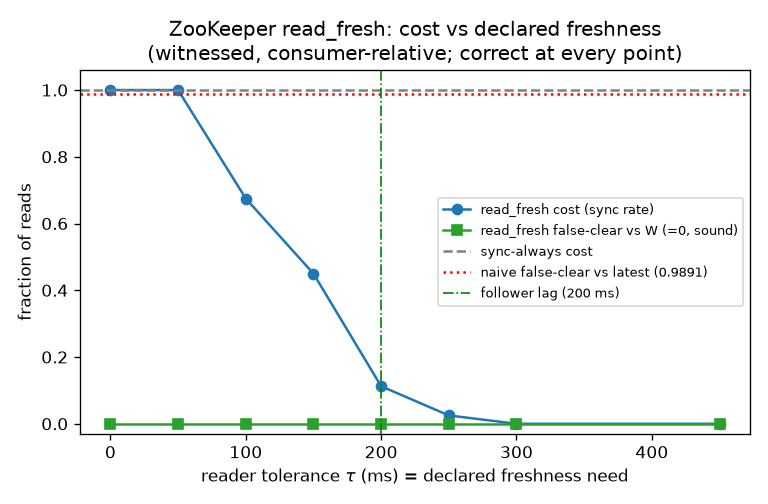
\includegraphics[width=\columnwidth]{zk-fix-cost-curve.png}
\caption{\texttt{read\_fresh} cost vs.\ the reader's declared tolerance $\tau$.
Cost (sync rate) is the follower-lag CDF; the false-clear against the reader's
watermark is zero throughout (the \texttt{zxid} is a sound witness). Naive and
\texttt{sync()}-always are the two blind endpoints.}
\label{fig:fix}
\end{figure}

Table~\ref{tab:uc} places the phenomenon and the fix in four real ZooKeeper
roles, drawn from a self-verifying use-case notebook that runs against the live
ensemble and asserts each outcome. A configuration reader (a cold footprint) is
served fresh locally; a service-discovery reader (a hot footprint) on the
\emph{same} follower is almost always stale; a bounded-staleness reader gets
guaranteed freshness at ${\sim}0.16$ sync cost; a leader/lock reader that needs
the latest correctly pays \texttt{sync()} on every read---and only it does.

\begin{table}[t]
\caption{Four ZooKeeper roles on the \emph{same} delayed follower, from the
self-verifying use-case notebook. Rows 1--2 are consumer-relativity; rows 3--4
are the fix.}
\label{tab:uc}\centering
\begin{tabular}{@{}L{3.4cm} C{1.5cm} C{1.5cm}@{}}
\toprule
role (footprint, policy) & stale / sync & false-clear \\
\midrule
config store (cold, naive)        & $0.033$ stale & --- \\
service discovery (hot, naive)    & $0.930$ stale & --- \\
bounded-staleness (\texttt{read\_fresh}, $\tau{=}$lag) & $0.156$ sync & $0.000$ \\
leader/lock (\texttt{read\_fresh}, $\tau{=}0$) & $1.000$ sync & $0.000$ \\
\bottomrule
\end{tabular}
\end{table}

\section{Discussion}
\emph{What this says about bounded-staleness reads.} Systems commonly expose a
staleness bound as a scalar (a lag threshold, a bounded-staleness read level).
The result argues that the useful bound is per-footprint and witnessed:
probabilistically bounded staleness~\cite{bailis2012pbs} calibrates the
distribution but globally; Spanner's commit-wait~\cite{corbett2012spanner} and
session guarantees~\cite{terry1994session} are witnessed or consumer-relative but
not jointly calibrated per footprint. The \texttt{zxid} already provides the
witness; the missing piece is to read $\PC$.

\emph{The broader program.} The same certificate/witness/false-clear grammar
recurs across substrates: WAL- and oplog-witnessed footprint certificates in
PostgreSQL and MongoDB, HARQ-witnessed adaptation certificates in 5G/6G radio
access, and BMP-witnessed reachability certificates in interdomain
routing~\cite{bond_ot}. ZooKeeper is the coordination-service case, and---because
its witness (\texttt{zxid}) and its correction (\texttt{sync()}) are already in
the protocol---the cleanest. Age of information~\cite{kaul2012aoi} bounds
staleness on the update channel; $\tr(\PC\Sigma)$ measures its consequence for a
specific reader, which is what a consistency SLA must bound. In CAP/PACELC
terms~\cite{gilbert2002cap,abadi2012pacelc}, the footprint certificate quantifies
the interior of the else-latency regime: it prices the consistency each reader
actually needs and pays latency (a \texttt{sync()}) only when the footprint
demands it.

\section{Limitations and Conclusion}
The measurement is a link-level ensemble with induced lag rather than a production
trace; watch-based reads, larger ensembles, and observer read-scaling are natural
extensions, and the footprint here is a set of znodes rather than a general read
operator. Within those bounds the conclusion is clean and, we hope, useful to
ZooKeeper's own users: a local read's freshness is a property of the reader's
footprint, not of the follower; the \texttt{zxid} is a sufficient witness; and
\texttt{sync()} is best understood as certifying the consumer's footprint. More
broadly, ZooKeeper is a particularly legible entry point to Observation
Theory---a system whose designers already built both the witness and the
correction the theory asks for.

\section*{Reproducibility}
The pre-registration, the coded verdict runner (with the cooling-off and
substrate guards), the ensemble scripts, the \texttt{read\_fresh} prototype, and
the graded record are archived with the program~\cite{bond_prereg}; the substrate
is unmodified ZooKeeper~3.9. A self-verifying use-case notebook
(\texttt{ZK-USE-CASES.ipynb}) stands up the ensemble, runs the four roles of
Table~\ref{tab:uc}, and \texttt{assert}s each outcome, so a clean run is a
passing suite.

\bibliographystyle{IEEEtran}
\bibliography{ot-replication-freshness}
\end{document}
